\documentclass[graybox]{svmult}
\usepackage{type1cm}
\usepackage{makeidx}
\usepackage{graphicx}
\usepackage{multicol}
\usepackage[bottom]{footmisc}
\usepackage{newtxtext} 
\usepackage[varvw]{newtxmath}
\makeindex

% AUTHOR MACROS
\usepackage{algpseudocode}
\usepackage{algorithm}
% \usepackage{listings}
% \lstdefinestyle{Python}{
%     showstringspaces = false,
%     language         = Python,
%     basicstyle       = \small\ttfamily,
%     morekeywords     = {as},
%     keywordstyle     = \color{black!70},
%     stringstyle      = \color{black!35},
%     commentstyle     = \color{black!35}\ttfamily,
% 	breaklines       = true,
% 	postbreak        = \text{$\hookrightarrow$\space},
% 	alsoletter       = {>,.},
%     morekeywords     = [2]{>>>,...},
%     keywordstyle     = [2]\color{black!70}\bfseries}
% \newcommand{\AGSComment}[1]{{\color{brown} #1}}
% \newcommand{\JRComment}[1]{{\color{violet}#1}}
% \newcommand{\FJHComment}[1]{{\color{purple}Fred:  #1}}
% \newcommand{\CDHJComment}[1]{{\color{royal blue}#1}}
% \usepackage{biblatex}
% \addbibresource{main.bib}
% \usepackage{natbib}
%\allowdisplaybreaks


\begin{document}
\title*{Monte Carlo for Vector Functions of Integrals}
\authorrunning{Sorokin \& Rathinavel}
\author{Aleksei G. Sorokin \and Jagadeeswaran Rathinavel}
\institute{
    Aleksei G. Sorokin \at Department of Applied Mathematics, Illinois Institute of Technology,\\ RE 220, 10 W.\ 32$^{\text{nd}}$ St., Chicago, IL 60616 \email{asorokin@hawk.iit.edu}
\and
    R. Jagadeeswaran \at Department of Applied Mathematics, Illinois Institute of Technology,\\ RE 220, 10 W.\ 32$^{\text{nd}}$ St., Chicago, IL 60616 \email{jrathin1@iit.edu}; and \\Wi-Tronix LLC, 631 E Boughton Rd, Suite 240, Bolingbrook, IL 60440}
\maketitle

\abstract{
Monte Carlo methods present an efficient approach for approximating the expected value of a random variable. Algorithms exist to adaptively sample the random variable until a user defined error tolerance is satisfied with high probability. This work describes an extension of such methods which supports adaptive sampling to satisfy error criteria for vector functions of multiple expectations. Although several functions involving multiple expectations are being evaluated, only one random sequence is required, albeit sometimes of larger dimension than the underlying randomness. These enhanced Monte Carlo and Quasi-Monte Carlo algorithms are implemented in the QMCPy Python package with support for vectorized, economical, and parallel function evaluation. We exemplify these capabilities on problems from machine learning and global sensitivity analysis.
}

\newpage

\section{Introduction}

Theoretical developments, stopping criteria, and implementations of Monte Carlo (MC) methods often focus on approximating a scalar expectation $\mu = \mathbb{E}[f(\boldsymbol{X})]$, where $\boldsymbol{X} \sim \mathcal{U}[0,1)^d$ encapsulates the randomness of a simulation $f: [0,1)^d \to \mathbb{R}$. However, many quantities of interest $\boldsymbol{s} \in \mathbb{R}^{\boldsymbol{d}_{\boldsymbol{s}}}$, which we call \emph{combined solutions}, may be formulated as functions of expectations $\boldsymbol{\mu} = \mathbb{E}[\boldsymbol{f}(\boldsymbol{X})] \in \mathbb{R}^{\boldsymbol{d}_{\boldsymbol{\mu}}}$, which we call \emph{individual solutions}. Now the simulation $\boldsymbol{f}: [0,1)^{d} \to \mathbb{R}^{\boldsymbol{d}_{\boldsymbol{\mu}}}$ produces a multi-dimensional array with shape vector $\boldsymbol{d}_{\boldsymbol{\mu}}$ for $\boldsymbol{X} \sim \mathcal{U}[0,1)^d$ as in the scalar function setting. The multi-dimensional array of combined solutions is produced from the multi-dimensional array of individual solutions via a \emph{combining function} $\boldsymbol{C}: \mathbb{R}^{\boldsymbol{d}_{\boldsymbol{\mu}}} \to \mathbb{R}^{\boldsymbol{d}_{\boldsymbol{s}}}$ so that $\boldsymbol{s} = \boldsymbol{C}(\boldsymbol{\mu})$.
For example, approximating
\begin{itemize}
    \item an $(a \times b)$ matrix of expectations may set $\boldsymbol{C}$ to the identity and $\boldsymbol{d}_{\boldsymbol{s}} = \boldsymbol{d}_{\boldsymbol{\mu}} = (a,b)$;
    \item the Bayesian posterior mean requires the ratio of expectations so that $s = C(\mu_1,\mu_2) = \mu_1/\mu_2$, $d_s = 1$, and $d_{\boldsymbol{\mu}} = 2$;
    \item $c$ closed and total sensitivity indices for global sensitivity analysis may require $\boldsymbol{d}_{\boldsymbol{s}} = (2,c)$ and $\boldsymbol{d}_{\boldsymbol{\mu}} = (2,3,c)$ to formulate $s_{ij} = C_{ij}(\boldsymbol{\mu}) =  \mu_{i3j}/(\mu_{i2j}-\mu_{i1j}^2)$ for $i \in \{1,2\}$ and $j \in \{1,\dots,c\}$.
\end{itemize}
These examples are further detailed in Section \ref{SoRa_sec:examples}.

This article generalizes \cite{adaptive_qmc} to develop Algorithm \ref{SoRa_algo:MCStoppingCriterion}, an efficient and adaptive method for approximating combined solutions $\boldsymbol{s}$ to within a user-specified error tolerance and uncertainty threshold. The algorithm utilizes existing MC  methods that, given an appropriate set of sampling nodes and their corresponding function evaluations, produce error bounds on individual solutions that hold with a desired confidence. Examples of scalar-bounding MC methods include \cite{cubmcg,cubqmclattice,cubqmcsobol,cubqmcbayes_thesis,cubqmcbayeslattice} with robust implementations in the GAIL MATLAB library \cite{ChoEtal21a,hickernell2018monte} among others. Interval arithmetic is used to propagate these individual solution bounds to bounds on the combined solutions which can be used both to test if the error criterion has been met and determine optimal combined solution approximations. 

Resulting vectorized MC algorithms for combined solutions are implemented into the open source QMCPy Python package \cite{QMCPy} which is distributed on both GitHub and PyPI. The implementations incorporate shared samples, multi-dimensional vectorization, parallel computation, and economical function evaluation to enable fast, efficient approximations.

The remainder of the article is organized as follows. Section \ref{SoRa_sec:MCM} provides a brief overview of scalar MC including both Crude and Quasi-MC methods. More detailed accounts of this mature field are available in \cite{niederreiter1992random,mcbook}. Section \ref{SoRa_sec:Existing_QMC_Methods} outlines various MC methods for determining error bounds on a scalar individual solution. Section \ref{SoRa_sec:comb_sol_approx} determines how to set uncertainty levels for individual bounds based on a desired uncertainty for a scalar combined solution and how to propagate bounds from individual to combined solutions using interval arithmetic \cite{interval_analysis}. Section \ref{SoRa_sec:opt_comb_sol_sc} derives a stopping criterion and optimal approximation for a scalar combined solution based on a user-specified uncertainty threshold and error metric map. Vectorization to a multi-dimensional array of combined solutions is described Section \ref{SoRa_sec: Vectorized Implementation} with consideration for economical function evaluation. This section also details Algorithm \ref{SoRa_algo:MCStoppingCriterion} which provides a framework for extending existing MC methods to accommodate approximating multi-dimensional arrays of combined solutions. Section \ref{SoRa_sec:examples} presents examples from machine learning and global sensitivity analysis before Section \ref{SoRa_sec:conclusions} concludes with with a brief summary.   

\section{Scalar Monte Carlo Methods} \label{SoRa_sec:MCM}

MC methods are well-suited to approximate a scalar expectation $\mu = \mathbb{E}[f(\boldsymbol{X})]$ where $\boldsymbol{X} \sim \mathcal{U}[0,1)^d$ contains the randomness of a simulation $f: [0,1)^{d} \to \mathbb{R}$. While the standard uniform choice for $\boldsymbol{X}$ may seem restrictive, a variety of random variables are compatible in this framework after an appropriate transformation. For example, if $\mu = \mathbb{E}[g(\boldsymbol{T})]$ for $\boldsymbol{T} \sim \mathcal{N}(\boldsymbol{m},\boldsymbol{\Sigma})$ and some $g: \mathbb{R}^{d} \to \mathbb{R}$, then $\mu = \mathbb{E}[f(\boldsymbol{X})]$ for  $f(\boldsymbol{x})=g(\boldsymbol{A}\boldsymbol{\Phi}^{-1}(\boldsymbol{x})+\boldsymbol{m})$ where $\boldsymbol{\Sigma}=\boldsymbol{A}\boldsymbol{A}^T$ and $\boldsymbol{\Phi}^{-1}$ is the inverse CDF of a standard normal distribution acting element wise. More details on such variable transformations can be found in \cite{QMCSoftware} along with examples of how to utilize the automatic transforms available in QMCPy.

MC methods often approximate $\mu$ by the sample average of $f$ evaluated at some nodes $\boldsymbol{x}_0,\dots,\boldsymbol{x}_{n-1} \in [0,1)^d$. We denote this approximation by  
\begin{equation}
    \label{SoRa_eq:mcapprox}
    \hat{\mu} = \frac{1}{n}\sum_{i=0}^{n-1} f(\boldsymbol{x}_i) \approx \mathbb{E}[f(\boldsymbol{X})] = \mu. 
\end{equation}
\emph{Crude Monte Carlo} (CMC) methods choose the sampling nodes to be independent and identically distributed (IID), that is $\boldsymbol{x}_0,\dots,\boldsymbol{x}_{n-1} \overset{\text{\tiny IID}}{\sim} \mathcal{U}[0,1)^{d}$. For CMC, the absolute approximation error $\lvert \mu - \hat{\mu} \rvert$ is $\mathcal{O}(n^{-1/2})$. 

\emph{Quasi-Monte Carlo} (QMC) methods choose the sampling nodes in a dependent manner to improve uniformity. Discrepancy measures quantify how close the empirical distribution of $\{\boldsymbol{x}_i\}_{i=0}^{n-1}$ is to the standard uniform distribution. The Koksma-Hlawka inequality bounds the absolute approximation error by the star discrepancy of $\{\boldsymbol{x}_i\}_{i=0}^{n-1}$ times the variation of $f$ in the sense of Hardy and Krause \cite{dick2013high}. Other discrepancy-variation pairings are also available, see \cite{hickernell1998generalized} for an overview. While it is often impractical to determine if $f$ has bounded variation, such inequalities indicate that using low discrepancy (LD) sequences in place of IID sequences can boost performance for nicely behaved $f$. A number of LD sequences exist that achieve a discrepancy of $\mathcal{O}(n^{-1+\delta})$ for any $\delta > 0$. These LD sequences are the backbone QMC methods. When $f$ has bounded variation, this rate upper bounds the absolute error of QMC methods making them significantly faster than CMC methods. Oftentimes, even if $f$ has infinite variation, QMC methods will still outperform CMC methods despite a lack of theoretical justification. 

The QMC methods in this article utilize randomized LD sequences that are extensible in both dimension and number of samples without sacrificing the $\mathcal{O}(n^{-1+\delta})$ discrepancy rate. Randomization ensures, with probability $1$, that $\boldsymbol{x}_0,\dots,\boldsymbol{x}_{n-1} \in (0,1)^d$ and that the LD sequence does not badly match the integrand. Extensiblity enables algorithms to adaptively increase the number of points used to estimate $\hat{\mu}$ without needing to discard previous function evaluations. Digital sequences and integration lattices are two popular choices for LD sequences. Constructions exist for both that support randomization and extensible designs. Figure \ref{SoRa_fig:ld_seqs} contrasts IID points with LD sequences implemented in base $2$ as is often done for computational efficiently.

\begin{figure}[t]
    \centering
    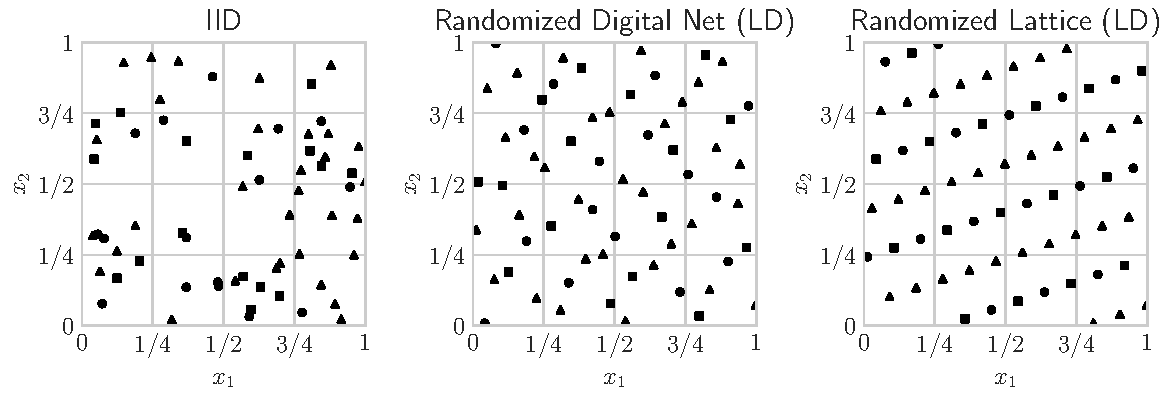
\includegraphics[width=\textwidth]{figs/ld_seqs.pdf}
    \caption{Contrast of IID points with randomized, extensible LD sequences. The first $2^4$ points of each sequence are squares, the next $2^4$ points are circles, and the $2^5$ points following that are triangles. Note the gaps and clusters in the IID sequence contrasted with the more even coverage of LD sequences. Also notice that as the sample size is doubled the extensible LD sequences fills in the gaps left by previous nodes.}
    \label{SoRa_fig:ld_seqs}
\end{figure}

\section{Scalar Monte Carlo Approximation Error}\label{SoRa_sec:Existing_QMC_Methods}

This section discusses some existing CMC and QMC methods for approximating error bounds on the scalar individual solution $\mu$. Specifically, given $n$ samples $\boldsymbol{x}_0,\dots,\boldsymbol{x}_{n-1}$ and corresponding function evaluations $f(\boldsymbol{x}_0),\dots,f(\boldsymbol{x}_{n-1})$, we discuss methods for determining a lower bound $\mu^-$ and upper bound $\mu^+$ so that $\mu \in [\mu^-,\mu^+]$ with probability greater than or equal to some desired threshold $1-\alpha^{(\mu)}$. Table \ref{SoRa_table:qmcpy_sc} compares the error bounding methods discussed in the remainder of this section.

\begin{table}[t]
\centering
\begin{tabular}{r c c c c c c}
    QMCPy Class Name & MC Type & Point Sets & Error Bounds \\
    \hline
    \texttt{CubMCCLT} \cite{cubmcg} & CMC & \texttt{IID} & Probabilistic \\
    \texttt{CubQMCRep} \cite{mcbook} & QMC & \texttt{LD} & Probabilistic \\
    \texttt{CubQMCNetG} \cite{cubqmcsobol} & QMC & \texttt{DigitalNetB2} & Deterministic \\
    \texttt{CubQMCLatticeG} \cite{cubqmclattice} & QMC & \texttt{Lattice} & Deterministic \\
    \texttt{CubQMCBayesNetG} \cite{cubqmcbayes_thesis} & QMC &  \texttt{DigitalNetB2} & Bayesian \\
    \texttt{CubQMCBayesLatticeG} \cite{cubqmcbayeslattice} & QMC & \texttt{Lattice} & Bayesian \\
    \hline
\end{tabular}
\caption{A comparison of select stopping criterion classes available in QMCPy. \emph{MC Type} indicates whether an algorithm is Crude Monte Carlo (CMC) or Quasi-Monte Carlo (QMC). \emph{Point Sets} indicate classes of compatible sequences in QMCPy. For example, \texttt{CubQMCRep} is compatible with any low discrepancy (\texttt{LD}) sequence including base 2 digital nets (\texttt{DigitalNetB2}) and integration lattices (\texttt{Lattice}). However, \texttt{CubQMCNetG} is only compatible with \texttt{DigitalNetB2} sequences and will not work with \texttt{Lattice} or other LD sequences. \emph{Error Bounds} specify the method of error estimation as discussed throughout this section. Deterministic error bounds hold with probability $1$ i.e. for any $\alpha^{(\mu)} \in (0,1)$. Probabilistic and Bayesian error bounds are tailored to the choice of $\alpha^{(\mu)}$.}
\label{SoRa_table:qmcpy_sc}
\end{table}

\begin{description}
    \item[\texttt{CubMCCLT}] When $\boldsymbol{x}_0,\dots,\boldsymbol{x}_{n-1}$ are IID and $f$ has finite variance, the Central Limit Theorem may provide a heuristic $1-\alpha^{(\mu)}$ confidence interval for $\mu$ by setting $\mu^\pm = \hat{\mu} \pm Z_{\alpha^{(\mu)}/2}\sigma/\sqrt{n}$. Here $Z_{\alpha^{(\mu)}/2}$ is the inverse CDF of a standard normal distribution at $1-\alpha^{(\mu)}/2$, and $\hat{\mu}$ is the sample average of function evaluations as in \eqref{SoRa_eq:mcapprox}. The variance of $f(\boldsymbol{X})$ is the generally unknown quantity $\sigma^2$ which may be approximated by the unbiased estimator $\hat{\sigma}^2 = 1/(n-1)\sum_{i=0}^{n-1}(f(\boldsymbol{x}_i)-\hat{\mu})^2$, perhaps multiplied by an inflation factor $C^2>1$ for a more conservative estimate. The resulting, heuristic error bounds on $\mu$ are $\mu^\pm = \hat{\mu} \pm CZ_{\alpha^{(\mu)}/2} \hat{\sigma} / \sqrt{n}$. These bounds only hold as $n \to \infty$ so they cannot be guaranteed to satisfy the desired uncertainty.
    
    Hickernell and collaborators build upon this idea in \cite{cubmcg} to accommodate  finite $n$ and provide error bounds that are guaranteed to satisfy the uncertainty threshold. Their two-step method relies on the Berry-Esseen inequality and the assumption that $f$ lies in a cone of functions with known, bounded kurtosis. This robust method is not immediately compatible with the framework of this article but has been implemented into the QMCPy stopping criterion class \texttt{CubMCG} to approximate a scalar individual solution.
    \item[\texttt{CubQMCRep}] This method utilizes IID randomizations of a LD sequence and then derives bounds based on the IID sample averages. Specifically, suppose $\{\boldsymbol{x}_i^{(1)}\}_{i=0}^{n-1},\dots,\{\boldsymbol{x}_i^{(R)}\}_{i=0}^{n-1}$ are $R$ IID randomizations of an LD point set. Then one may compute the $R$ IID sample averages $\hat{\mu}_r = \frac{1}{n} \sum_{i=0}^{n-1} f(\boldsymbol{x}_i^{(r)})$ for $r = 1,\dots,R$. Similar to what was done for \texttt{CubMCCLT}, one may then compute $\hat{\mu} = 1/R \sum_{r=1}^R \hat{\mu}_r$ and $\hat{\sigma}_R = \sqrt{1/(R-1)\sum_{i=1}^R(\hat{\mu}_r - \hat{\mu})^2}$ to produce heuristic bounds $\mu^\pm = \hat{\mu} \pm \frac{C T_{\alpha^{(\mu)}/2,R-1} \hat{\sigma}_R}{\sqrt{R}}$. Here $C>1$ is still an inflation factor and we now use $T_{\alpha^{(\mu)}/2,R-1}$, the inverse CDF of Student's-$t$ distribution with $R-1$ degrees of freedom, instead of $Z_{\alpha^{(\mu)}/2}$.
    A more careful treatment of this heuristic method is available in either \cite[Chapter 17]{mcbook} or \cite{qmc4pde}. 
    \item[\texttt{CubQMC\{Net,Lattice\}G}] Hickernell and Rugama developed algorithms in \cite{adaptive_qmc} that track the decay of Fourier coefficients based on a single randomized LD sequence i.e. $R=1$. These algorithms provide deterministic error bounds on $\mu$ for functions in a cone parameterized by the decay rate of the Walsh coefficients for digital sequences \cite{cubqmcsobol} or the complex exponential Fourier coefficients for integration lattices \cite{cubqmclattice}. 
    \item[\texttt{CubQMCBayes\{Net,Lattice\}G}] Another pair of QMC algorithms take a Bayesian approach to error estimation, again using only a single randomized LD sequence. Rather than assume the function lies within a cone, these algorithms assume the integrand is an instance of a Gaussian process. Utilizing special kernels matched to LD sequences allows fast approximation of Gaussian process hyperparameters and provides tractable error estimation. These Bayesian QMC algorithms are also available for both digital nets \cite{cubqmcbayes_thesis} and integration lattices  \cite{cubqmcbayeslattice}. 
    %Similar to \texttt{CubQMC\{Net,Lattice\}G}, Fourier and Walsh transform coefficients are used respectively with Lattice and digital nets. But the coefficients are used to estimate credible intervals. Thus it provides much stronger theoretical background. These algorithms need to estimate shape and scale parameters to parameterize the covariance kernels, which are to be searched using optimization techniques, leading to greater computational cost. 
\end{description}

We first recommend using the  \texttt{CubQMC\{Net,Lattice\}G} QMC algorithms if the function's Fourier coefficients are expected to be well behaved and the function has low evaluation cost. For functions with larger evaluation cost and low dimension, we recommend using  \texttt{CubQMCBayes\{Net,Lattice\}G}. While these algorithms require additional overhead for optimizing Gaussian Process hyperparameters, they tend to be more sample efficient than \texttt{CubQMC\{Net,Lattice\}G}. \texttt{CubQMCRep} accommodates a larger class of functions compared to the other QMC algorithms with the drawback of providing heuristic bounds and often requiring more samples to achieve the same error. If QMC is not suitable for the problem, \texttt{CubMCCLT} may be used, again with the caution of producing heuristic bounds which lack theoretical justification.

Digital net schemes may be preferred to lattice schemes as the later often requires the function be periodic. While periodizing transforms are available to any function, such transforms may destroy smoothness properties previously enjoyed by the function. See \cite[Chapter 16]{mcbook} for more details on periodizing transforms for lattice rules.

\section{Bounds on a Scalar Combined Solution} \label{SoRa_sec:comb_sol_approx}

In this section, we connect errors in individual solutions to error in a combined solution. The MC and QMC algorithms in the previous section may be vectorized in a straightforward manner to attain error bounds $[\boldsymbol{\mu}^-,\boldsymbol{\mu}^+]$ on a multi-dimensional array of individual solutions $\boldsymbol{\mu} \in \mathbb{R}^{\boldsymbol{d}_{\boldsymbol{\mu}}}$ so that 
\begin{equation}
    P(\mu_{\boldsymbol{k}} \in [\mu_{\boldsymbol{k}}^-,\mu_{\boldsymbol{k}}^+]) \geq 1-\alpha_{\boldsymbol{k}}^{(\boldsymbol{\mu})}  \qquad \text{for any multi-index }\boldsymbol{1} \leq \boldsymbol{k} \leq \boldsymbol{d}_{\boldsymbol{\mu}}.
    \label{SoRa_eq:indv_prob_bounds}
\end{equation}
Here $\boldsymbol{\alpha}^{(\boldsymbol{\mu})} \in (0,1)^{\boldsymbol{d}_{\boldsymbol{\mu}}}$ is a multi-dimensional array of individual uncertainty levels which are set to 
\begin{equation}
    \alpha_{\boldsymbol{k}}^{(\boldsymbol{\mu})} = \frac{\alpha^{(s)}}{\prod(\boldsymbol{d}_{\boldsymbol{\mu}})}
    \label{SoRa_eq:alpha_mu_from_alpha_s} \qquad \text{for all }\boldsymbol{1} \leq \boldsymbol{k} \leq \boldsymbol{d}_{\boldsymbol{\mu}}.
\end{equation}
In the above, $\prod(\boldsymbol{d}_{\boldsymbol{\mu}})$ is the product of all entries in $\boldsymbol{d}_{\boldsymbol{\mu}}$, i.e. the number of elements in a $\mathbb{R}^{\boldsymbol{d}_{\boldsymbol{\mu}}}$ array, and $\alpha^{(s)} \in (0,1)$ is the desired uncertainty for the bounds $[s^-,s^+]$ on the scalar combined solution $s$. Under this setting, Boole's inequality \cite{boole1847mathematical} implies that whenever \eqref{SoRa_eq:indv_prob_bounds} holds we have
\begin{equation}
    P(\boldsymbol{\mu} \in [\boldsymbol{\mu}^-,\boldsymbol{\mu}^+]) \geq 1-\alpha^{(s)}.
    \label{SoRa_eq:indv_prob_bounds_all}
\end{equation} 

Recall that $s = C(\boldsymbol{\mu})$ where $C: \mathbb{R}^{\boldsymbol{d}_{\boldsymbol{\mu}}} \to \mathbb{R}$. To propagate individual bounds $[\boldsymbol{\mu}^-,\boldsymbol{\mu}^+]$ to combined bounds $[s^-,s^+]$, one defines interval arithmetic \cite{interval_analysis} functions $C^-,C^+: \mathbb{R}^{\boldsymbol{d}_{\boldsymbol{\mu}}} \times \mathbb{R}^{\boldsymbol{d}_{\boldsymbol{\mu}}} \to \mathbb{R}$ so that
\begin{equation}
    s^- = C^-(\boldsymbol{\mu}^-,\boldsymbol{\mu}^+) = \min_{\boldsymbol{\mu} \in [\boldsymbol{\mu}^-,\boldsymbol{\mu}^+]} C(\boldsymbol{\mu}), \quad 
    s^+= C^+(\boldsymbol{\mu}^-,\boldsymbol{\mu}^+) = \max_{\boldsymbol{\mu} \in [\boldsymbol{\mu}^-,\boldsymbol{\mu}^+]} C(\boldsymbol{\mu}).
    \label{SoRa_eq:C_minus_C_plus}
\end{equation}
Table \ref{SoRa_table:elementary_ops_Cpm} provides examples of such interval arithmetic functions for some basic operations. In all, given combined uncertainty threshold $\alpha^{(s)}$ we may set individual thresholds $\boldsymbol{\alpha}^{(\boldsymbol{\mu})}$ via \eqref{SoRa_eq:alpha_mu_from_alpha_s} then use vectorized, scalar MC algorithms to find individual bounds $[\boldsymbol{\mu}^-,\boldsymbol{\mu}^+]$ satisfying \eqref{SoRa_eq:indv_prob_bounds} so that \eqref{SoRa_eq:indv_prob_bounds_all} holds. Then setting combined bounds $[s^-,s^+]$ via \eqref{SoRa_eq:C_minus_C_plus} will guarantee we satisfy the desired inequality 
$$P(s \in [s^-,s^+]) \geq 1-\alpha^{(s)}.$$

\begin{table}[t]
\begin{tabular}{r  c  c}
    $s=C(\boldsymbol{\mu})$ & $s^- = C^-(\boldsymbol{\mu}^-,\boldsymbol{\mu}^+)$ & $s^+ = C^+(\boldsymbol{\mu}^-,\boldsymbol{\mu}^+)$ \\
    \hline
    $\mu_1+\mu_2$ & $\mu_1^-+\mu_2^-$ & $\mu_1^++\mu_2^+$ \\
    $\mu_1-\mu_2$ & $\mu_1^--\mu_2^+$ & $\mu_1^+-\mu_2^-$ \\
    $\mu_1 \cdot \mu_2$ & $\min(\mu_1^-\mu_2^-,\mu_1^-\mu_2^+,\mu_1^+\mu_2^-,\mu_1^+\mu_2^+)$ & $\max(\mu_1^-\mu_2^-,\mu_1^-\mu_2^+,\mu_1^+\mu_2^-,\mu_1^+\mu_2^+)$ \\
    $\mu_1 / \mu_2$ & $\begin{cases} -\infty, & 0 \in [\mu_2^-,\mu_2^+] \\ \min\left(\frac{\mu_1^-}{\mu_2^-},\frac{\mu_1^+}{\mu_2^-},\frac{\mu_1^-}{\mu_2^+},\frac{\mu_1^+}{\mu_2^+}\right), & 0 \notin [\mu_2^-,\mu_2^+] \end{cases}$ & $\begin{cases} \infty, & 0 \in [\mu_2^-,\mu_2^+] \\ \max\left(\frac{\mu_1^-}{\mu_2^-},\frac{\mu_1^+}{\mu_2^-},\frac{\mu_1^-}{\mu_2^+},\frac{\mu_1^+}{\mu_2^+}\right), & 0 \notin [\mu_2^-,\mu_2^+] \end{cases}$ \\
    $\min(\mu_1,\mu_2)$ & $\min(\mu_1^-,\mu_2^-)$ & $\min(\mu_1^+,\mu_2^+)$ \\
    $\max(\mu_1,\mu_2)$ & $\max(\mu_1^-,\mu_2^-)$ & $\max(\mu_1^+,\mu_2^+)$ \\
    \hline
\end{tabular}
\caption{Bound propagation functions for elementary operations on individual solutions.}
\label{SoRa_table:elementary_ops_Cpm}
\end{table}

\section{Optimal Approximation of a Scalar Combined Solution} \label{SoRa_sec:opt_comb_sol_sc}

This section derives a stopping criterion and optimal approximation for a scalar combined solution. Let $h^{(\varepsilon)}: \mathbb{R} \to \mathbb{R}^+$ be an error metric dependent on some error threshold $\varepsilon$ so that the stopping criterion is met if and only if the combined solution approximation $\hat{s}$ satisfies 
\begin{equation}
    \lvert s-\hat{s} \rvert \leq h^{(\varepsilon)}(s) \qquad \text{for all } s \in [s^-,s^+].
    \label{SoRa_eq:sc_raw}
\end{equation}
Theorem \ref{SoRa_thm:shat_opt} below determines an optimal $\hat{s}$ and an equivalent condition to \eqref{SoRa_eq:sc_raw} when $h^{(\varepsilon)}$ is a metric map i.e Lipschitz continuous with constant at most $1$. Some compatible error metric options are
\begin{subequations}
\begin{align}
    h^{(\varepsilon)}(s) &= \max\left(\varepsilon^\text{abs},\lvert s \rvert \varepsilon^\text{rel} \right) \quad &&\text{absolute or relative error satisfied,} \label{SoRa_eq:h_abs_or_rel} \\
    h^{(\varepsilon)}(s) &= \min\left(\varepsilon^\text{abs},\lvert s \rvert \varepsilon^\text{rel} \right) \quad &&\text{absolute and relative error satisfied.} \label{SoRa_eq:h_abs_and_rel}
\end{align}
\end{subequations}
\begin{theorem} \label{SoRa_thm:shat_opt}
    Suppose that  $h^{(\varepsilon)}$ satisfies the metric map condition
    \begin{equation}
        \lvert h^{(\varepsilon)}(s_1) - h^{(\varepsilon)}(s_2) \rvert \leq \lvert s_1 - s_2 \rvert \qquad \text{for all } s_1,s_2 \in \mathbb{R}.
        \label{SoRa_eq:metric_map_cond}
    \end{equation}
    Then error criterion  \eqref{SoRa_eq:sc_raw} holds if and only if 
    \begin{equation}
        s^+-s^- \leq h^{(\varepsilon)}(s^-)+h^{(\varepsilon)}(s^+).
        \label{SoRa_eq:sc}
    \end{equation}
    Furthermore, the choice of 
    \begin{equation}
        \hat{s} = \frac{1}{2}\left[s^-+s^++h^{(\varepsilon)}(s^-)-h^{(\varepsilon)}(s^+)\right]
        \label{SoRa_eq:shat_opt}
    \end{equation}
    minimizes $\max_{s \in [s^-,s^+]} \lvert s - \hat{s} \rvert -h^{(\varepsilon)}(s)$ for any choice of $s^{\pm}$ with $s^- < s^+$.
\end{theorem}

\begin{proof}
    Define $g(s,\hat{s})=\lvert s - \hat{s} \rvert -h^{(\varepsilon)}(s)$. From \eqref{SoRa_eq:metric_map_cond}, it follows that if  $s^- \leq s \leq \hat{s}$ then $g(s^-,\hat{s})-g(s,\hat{s}) \geq 0$, and if $\hat{s} \leq s \leq s^+$ then $g(s^+,\hat{s})-g(s,\hat{s})  \geq 0$. This means that $g(\cdot,\hat{s})$ attains its maximum at either $s^-$ or $s^+$ so that
    \begin{equation*}
        \max_{s \in [s^-,s^+]} g(s,\hat{s}) = \max_{s \in \{s^-,s^+\}} g(s,\hat{s}).
    \end{equation*}
    
    Next, we find the optimal choice of $\hat{s}$.  The function $g(s^-,\cdot)$ is monotonically decreasing to the left of  $s^-$ and monotonically increasing to the right of $s^-$. Similarly, $g(s^+,\cdot)$ is monotonically decreasing to the left of $s^+$ and monotonically increasing to the right of $s^+$. This means that the optimal choice of $\hat{s}$ to minimize $\max_{s \in \{s^-,s^+\}} g(s,\hat{s})$ lies in $[s^-,s^+]$ and satisfies $g(s^-,\hat{s}) = g(s^+,\hat{s})$, that is, 
    $$\hat{s} - s^- - h^{(\varepsilon)}(s^-) = s^+ - \hat{s} - h^{(\varepsilon)}(s^+).$$
    Solving for the optimal value of $\hat{s}$ leads to \eqref{SoRa_eq:shat_opt}.
    
    For this optimal $\hat{s}$, 
    $$2 \max_{s \in [s^-,s^+]} g(s,\hat{s}) =  s^+  -  s^-  - h^{(\varepsilon)}(s^-) - h^{(\varepsilon)}(s^+).$$
    The error criterion is equivalent to $\max_{s \in [s^-,s^+]} g(s,\hat{s}) \le 0 $.  This can only hold under condition  \eqref{SoRa_eq:sc}. 
\end{proof}

\section{Fully Vectorized (Quasi-)Monte Carlo Algorithm} \label{SoRa_sec: Vectorized Implementation}

In the previous section we assumed that a multi-dimensional array of individual solutions $\boldsymbol{\mu} \in \mathbb{R}^{\boldsymbol{d}_{\boldsymbol{\mu}}}$ were used to compute a scalar combined solution $s \in \mathbb{R}$. We now relax these assumptions to enable approximation of multi-dimensional combined solutions $\boldsymbol{s} \in \mathbb{R}^{\boldsymbol{d}_{\boldsymbol{s}}}$. The optimal approximation $\hat{\boldsymbol{s}} \in \mathbb{R}^{\boldsymbol{d}_{\boldsymbol{s}}}$ and stopping criterion may still be computed by element wise versions of \eqref{SoRa_eq:shat_opt} and \eqref{SoRa_eq:sc}. 

To enable economical function evaluation, the user may define a dependency function $\boldsymbol{D}: \{\text{True},\text{False}\}^{\boldsymbol{d}_{\boldsymbol{s}}} \to \{\text{True},\text{False}\}^{\boldsymbol{d}_{\boldsymbol{\mu}}}$ which maps error criterion flags on combined solutions to flags on individual solutions. These individual flags indicate which outputs the integrand is required to compute in the next iteration. Take a simple example where  $\boldsymbol{s}=\boldsymbol{\mu}$, so $\boldsymbol{C}$ and $\boldsymbol{D}$ are the identity function. At some iteration suppose the combined flag at multi-index $\boldsymbol{1} \leq \boldsymbol{l} \leq \boldsymbol{d}_{\boldsymbol{s}}$ is $\text{True}$, indicating the combined, and therefore individual, solution at index $\boldsymbol{l}$ has been sufficiently approximated. Then in the next iteration, the function does not need to compute outputs at index $\boldsymbol{l}$.

Moreover, $\boldsymbol{D}$ may be used to compute individual uncertainty levels $\boldsymbol{\alpha}^{(\boldsymbol{\mu})}$ by determining which and how many individual solution contribute to a combined solution. Specifically, we may adapt \eqref{SoRa_eq:alpha_mu_from_alpha_s} so that 
$\alpha_{\boldsymbol{k}}^{(\boldsymbol{\mu})}$ is the reciprocal of the maximum number of dependent individual solutions across all combined solutions which include an index $\boldsymbol{k}$ dependency.

Algorithm \ref{SoRa_algo:MCStoppingCriterion} details the adaptive, vectorized MC procedure developed throughout this article. Notice that the implementation does not require specifying $\boldsymbol{C}$ despite its use in deriving the necessary $\boldsymbol{C}^-,\boldsymbol{C}^+$ inputs. The cost of this algorithm is concentrated in evaluating the function at an IID or LD sequence. In practice, the run time may be reduced if the users simulation code can take advantage of not having to compute all outputs at every iteration or through parallel evaluation if the simulation is costly to evaluate.

\begin{algorithm}[t]
    \caption{Adaptive, Vectorized (Quasi-)Monte Carlo Algorithm}
    \label{SoRa_algo:MCStoppingCriterion}
    \begin{algorithmic}
    \Require $\boldsymbol{f}: (0,1)^d \to \mathbb{R}^{\boldsymbol{d}_{\boldsymbol{\mu}}}$, the simulation where $\boldsymbol{\mu} = \mathbb{E}[\boldsymbol{f}(\boldsymbol{X})]$ for $\boldsymbol{X} \sim \mathcal{U}[0,1)^d$.
    \Require $\boldsymbol{\alpha}^{(\boldsymbol{s})} \in (0,1)^{\boldsymbol{d}_{\boldsymbol{s}}}$, the desired uncertainty levels for combined solutions so $[\boldsymbol{s}^-,\boldsymbol{s}^+]$ satisfy $P(s_{\boldsymbol{l}} \in [s_{\boldsymbol{l}}^-,s_{\boldsymbol{l}}^+]) \geq 1-\alpha^{(\boldsymbol{s})}_{\boldsymbol{l}}$ for any $\boldsymbol{1} \leq \boldsymbol{l} \leq \boldsymbol{d}_{\boldsymbol{s}}$. If the user wants bounds $[\boldsymbol{s}^-,\boldsymbol{s}^+]$ to satisfy $P(\boldsymbol{s} \in [\boldsymbol{s}^-,\boldsymbol{s}^+]) \geq 1-\alpha$ for some $\alpha \in (0,1)$ then set $\alpha_{\boldsymbol{l}}^{(\boldsymbol{s})} = 1/\prod(\boldsymbol{d}_{\boldsymbol{s}})$ in the spirit of \eqref{SoRa_eq:alpha_mu_from_alpha_s}.
    \Require $\boldsymbol{C}^-,\boldsymbol{C}^+: \mathbb{R}^{\boldsymbol{d}_{\boldsymbol{\mu}}} \times \mathbb{R}^{\boldsymbol{d}_{\boldsymbol{\mu}}} \to \mathbb{R}^{\boldsymbol{d}_{\boldsymbol{s}}}$, vectorized interval arithmetic functions as in \eqref{SoRa_eq:C_minus_C_plus}.
    \Require $h^{(\varepsilon_{\boldsymbol{l}})}_{\boldsymbol{l}}: \mathbb{R} \to \mathbb{R}^+$ for $\boldsymbol{1} \leq \boldsymbol{l} \leq \boldsymbol{d}_{\boldsymbol{l}}$. See \eqref{SoRa_eq:h_abs_or_rel} or \eqref{SoRa_eq:h_abs_and_rel} for examples.
    \Require $\boldsymbol{D}: \{\text{True},\text{False}\}^{\boldsymbol{d}_{\boldsymbol{s}}} \to \{\text{True},\text{False}\}^{\boldsymbol{d}_{\boldsymbol{\mu}}}$, a dependency function mapping stopping criterion flags for the combined solutions to flags for individual solutions. 
    \Require A scalar CMC or QMC algorithm capable of producing bounds on an individual solution which hold with desired uncertainty. See the methods in Section \ref{SoRa_sec:Existing_QMC_Methods}.
    \Require A generator of IID or LD sequences compatible with the scalar CMC or QMC algorithm. 
    \Require $m_0 \in \mathbb{N}$, where $2^{m_0}$ is the initial number of samples.
    \\ \hrulefill
    \State $n_\text{start} \gets 0$ \Comment{lower index in node sequence(s)}
    \State $n_\text{end} \gets 2^{m_0}$ \Comment{upper index in node sequence(s), \emph{not} inclusive}
    \State $\boldsymbol{b}^{(\boldsymbol{\mu})} \gets \text{False}^{\boldsymbol{d}_{\boldsymbol{\mu}}}$ \Comment{flags on individual solutions}
    \State $\boldsymbol{b}^{(\boldsymbol{s})} \gets \text{False}^{\boldsymbol{d}_{\boldsymbol{s}}}$ \Comment{flags on combined solutions}
    \State Set $\boldsymbol{\alpha}^{(\boldsymbol{\mu})}$ based on $\boldsymbol{\alpha}^{(\boldsymbol{s})}$ as described in Section \ref{SoRa_sec: Vectorized Implementation}
    \While{$b_{\boldsymbol{l}}^{(\boldsymbol{s})} = \text{False}$ for some $\boldsymbol{1} \leq \boldsymbol{l} \leq \boldsymbol{d}_{\boldsymbol{s}}$} \Comment{A combined solution is not sufficiently bounded}
        \State Generate nodes from the IID or LD sequence(s) from index $n_\text{start}$ to $n_\text{end}-1$
        \State Evaluate $\boldsymbol{f}$ at the new nodes where $\boldsymbol{b}^{(\boldsymbol{\mu})}=\textbf{\text{False}}$ \Comment{may be done in parallel}
        \State Update $\boldsymbol{\mu}^-$ and $\boldsymbol{\mu}^+$ using the scalar CMC or QMC algorithms where $\boldsymbol{b}^{(\boldsymbol{\mu})}=\textbf{\text{False}}$
        \State $[\boldsymbol{s}^-,\boldsymbol{s}^+] = \left[\boldsymbol{C}^-(\boldsymbol{\mu}^-,\boldsymbol{\mu}^+),\boldsymbol{C}^+(\boldsymbol{\mu}^-,\boldsymbol{\mu}^+)\right]$ 
        \State $\hat{s}_{\boldsymbol{l}} \gets \frac{1}{2}\left[s_{\boldsymbol{l}}^-+s_{\boldsymbol{l}}^++h^{(\varepsilon_{\boldsymbol{l}})}_{\boldsymbol{l}}(s_{\boldsymbol{l}}^-)-h^{(\varepsilon_{\boldsymbol{l}})}_{\boldsymbol{l}}(s_{\boldsymbol{l}}^+)\right], \quad\boldsymbol{1} \leq \boldsymbol{l} \leq \boldsymbol{d}_{\boldsymbol{s}}$ \Comment{\eqref{SoRa_eq:shat_opt} element wise}
        \State $b^{(\boldsymbol{s})}_{\boldsymbol{l}} \gets \text{Boolean}\left(s_{\boldsymbol{l}}^+-s_{\boldsymbol{l}}^- < h^{(\varepsilon_{\boldsymbol{l}})}_{\boldsymbol{l}}(s_{\boldsymbol{l}}^-)+h^{(\varepsilon_{\boldsymbol{l}})}_{\boldsymbol{l}}(s_{\boldsymbol{l}}^+)\right),\quad \boldsymbol{1} \leq \boldsymbol{l} \leq \boldsymbol{d}_{\boldsymbol{s}}$ \Comment{\eqref{SoRa_eq:sc} element wise}
        \State $\boldsymbol{b}^{(\boldsymbol{\mu})} \gets \boldsymbol{D}\left(\boldsymbol{b}^{(\boldsymbol{s})}\right)$
        \State $n_\text{start} \gets n_\text{end}$
        \State $n_\text{end} \gets 2n_\text{start}$
    \EndWhile
    \State \Return $\hat{\boldsymbol{s}},[\hat{\boldsymbol{s}}^-,\hat{\boldsymbol{s}}^+]$
    \end{algorithmic}
\end{algorithm}

\section{Examples} \label{SoRa_sec:examples}

This section presents a number of examples spanning machine learning and sensitivity analysis. Code implementing these examples in the QMCPy framework and reproducing the figures in this article is available in \cite{vectorized_qmc_demo_notebook}. For more details on using QMCPy for scalar individual solution approximation see \cite{QMCSoftware}.

% Throughout the remainder of this section we assume the QMCPy package \cite{QMCPy} has been imported alongside the numerical package NumPy \cite{numpy} via the following Python commands:
% \lstinputlisting[style=Python,label={py:imports}]{python/imports.txt}
% The four main abstract classes in QMCPy are the 
% \begin{itemize}
%     \item \emph{discrete distribution} class for generating IID or LD sequences;
%     \item \emph{true measure} class for facilitating variable transforms to adapt randomness to the standard uniform;
%     \item \emph{integrand} class specifying the function of the true measure we want to take the expectation of; 
%     \item \emph{stopping criterion} class with an \texttt{integrate} method to adaptively sample the integrand until the stopping criterion is satisfied as in Algorithm \ref{SoRa_algo:MCStoppingCriterion}.
% \end{itemize}
% Each MC problem must instantiate a subclass of each of the four abstract classes in a nested fashion. 

% As a simple example, let us compute the expected displacement and stress on a cantilever beam as defined in \cite{ simulationlib_cantilever}: 
% \begin{equation*}
%     D(T_1,T_2,T_3) = \frac{4l^3}{T_1 w t} \sqrt{\frac{T_2^2}{t^4} + \frac{T_3^2}{w^4}}, \qquad S(T_1,T_2,T_3) = 600\left(\frac{T_2}{wt^2} + \frac{T_3}{w^2t}\right).
%     \label{SoRa_eq:cantilever_beam}
% \end{equation*}
% Here $l=100$, $w=4$, $t=2$ are constants and $T_1$, $T_2$, $T_3$ are independent Gaussian random variables with mean and standard deviation as defined as in the Table \ref{tab:cantilever_beam} below.
% \begin{table}[t]
%     \centering
%     \begin{tabular}{r c c l}
%         Gaussian Variable & mean & standard deviation & Description \\ 
%         \hline \\
%         $T_1$ & $2.9 \times 10^7$ & $1.45 \times 10^6$ & Young's modulus of beam material \\
%         $T_2$ & $500$ & $100$ & horizontal load on beam \\
%         $T_3$ & $1000$ & $100$ & vertical load on beam
%     \end{tabular}
%     \caption{Variable descriptions for the cantilever beam function.}
%     \label{tab:cantilever_beam}
% \end{table}
% Listing \ref{py:simpleex} uses QMCPy to approximates $s_1 = \mu_1 = \mathbb{E}[D(\boldsymbol{T})]$ and $s_2 = \mu_2 = \mathbb{E}[S(\boldsymbol{T})]$ where the identity functions for $\boldsymbol{C}^-$, $\boldsymbol{C}^+$, and $\boldsymbol{D}$ are defaulted to. Notice that \texttt{CustomFun} is initialized with $g=(D,S)$ as a function of the Gaussian random vector $\boldsymbol{T}$ rather than the transformed integrand $f$, which is a function of $\boldsymbol{X} \sim \mathcal{U}(0,1)^3$. The variable transform taking $g$ to $f$ is performed automatically by QMCPy without explicit specification from the user. Here the default absolute or relative error metric \eqref{SoRa_eq:h_abs_or_rel} is used.
% \lstinputlisting[caption={Simple QMCPy Example},style=Python,label={py:simpleex}]{python/simple_ex.txt}

\subsection{Vectorized Acquisition Functions for Bayesian Optimization}

Bayesian optimization (BO) is a sequential optimization technique that attempts to find the global maximum of a black box function $\varphi: (0,1)^{\nu} \to \mathbb{R}$. It is assumed that $\varphi$ is expensive to evaluate, so we must strategically select sampling locations that maximize some utility or acquisition function. At a high level, BO 
\begin{enumerate}
    \item iteratively samples $\varphi$ at locations maximizing the acquisition function,
    \item updates a Gaussian process surrogate based on these new observations,
    \item updates an acquisition function based on the updated surrogate,
    \item and repeats until the budget for sampling $\varphi$ has been expired.
\end{enumerate}
More details on Bayesian optimization including formulas for the posterior mean and covariance of a Gaussian Process may be found in \cite{frazier2018tutorial}.

Concretely, suppose we have already sampled $\varphi$ at $\boldsymbol{z}_1,\dots,\boldsymbol{z}_{N} \in [0,1]^{\nu}$ to collect data $\mathcal{D}=\{(\boldsymbol{z}_i,y_i)\}_{i=1}^N$ where $y_i = \varphi(\boldsymbol{z}_i)$. BO may then fit a Gaussian process surrogate to data $\mathcal{D}$. The next $q$ sampling locations may then be chosen to maximize an acquisition function $\alpha$ based on the surrogate so that $\boldsymbol{z}_{N+1}, \dots, \boldsymbol{z}_{N+q}$ are the rows of $\mathop{\text{argmax}}_{\boldsymbol{Z} \in [0,1]^{(q,d)}}\alpha(\boldsymbol{Z})$. Many acquisition functions may be expressed as an expectation of the form $\alpha(\boldsymbol{Z}) = \mathbb{E}\left[a(\boldsymbol{y}) \mid \boldsymbol{y} \sim \mathcal{N}\left(\boldsymbol{m},\boldsymbol{\Sigma}\right)\right]$ where $\boldsymbol{m} \in \mathbb{R}^{q}$, $\boldsymbol{\Sigma} \in \mathbb{R}^{(q, q)}$ are the posterior mean, covariance of the Gaussian process at points $\boldsymbol{Z}$. Here we focus on the q-Expected Improvement (QEI) acquisition function which uses $a(\boldsymbol{y}) = \max_{1 \leq i \leq q} (y_i - y^*)_+$ where $y^*= \max\left(y_1,\dots,y_N\right)$ is the current maximum and $(\cdot)_+ = \max(\cdot,0)$. 

Suppose we choose the argument maximum  from among a finite set of $q$-sized batches $\boldsymbol{Z}_1,\dots,\boldsymbol{Z}_c \in [0,1]^{(q, d)}$ so that $\boldsymbol{z}_{N+1}, \dots,\boldsymbol{z}_{N+q}$ are set to be the rows of $\mathop{\text{argmax}}_{\boldsymbol{Z} \in \{\boldsymbol{Z}_1,\dots,\boldsymbol{Z}_c\}}\alpha(\boldsymbol{Z})$. We may vectorize the acquisition function computations to $s_i = \mu_i = \alpha(\boldsymbol{Z}_i) = \mathbb{E}\left[a\left(\boldsymbol{A}_i\boldsymbol{\Phi}^{-1}(\boldsymbol{X})+\boldsymbol{m}_i\right)\right]$ for $i=1,\dots,c$ where $\boldsymbol{X} \sim \mathcal{U}(0,1)^q$ and $\boldsymbol{\Phi}^{-1}$ is the inverse CDF of the standard Gaussian taken element wise. Now $\boldsymbol{m}_i$, $\boldsymbol{\Sigma}_i = \boldsymbol{A}_i\boldsymbol{A}_i^T$ are the posterior mean, covariance respectively of the Gaussian process at $\boldsymbol{Z}_i$ so that $\boldsymbol{A}_i\boldsymbol{\Phi}^{-1}(\boldsymbol{X})+\boldsymbol{m}_i \sim \mathcal{N}\left(\boldsymbol{m}_i,\boldsymbol{\Sigma}_i\right)$ for $i=1,\dots,c$.

Since the quantity of interest is simply the vector of expectations, one may set $\boldsymbol{C}$, $\boldsymbol{C}^-$, $\boldsymbol{C}^+$, and $\boldsymbol{D}$ to appropriate identity functions. The process described above is visualized in Figure \ref{SoRa_fig:bo_qei} for $d=1$ and $q=2$. Notice the optimal next points trade off exploiting parts of the domain where performant samples have already been observed and  exploring parts of the domain where the Gaussian Process has large uncertainty.  As $q$ and/or $d$ grow, the number of candidates $c$ required for the discrete argument maximum to be a good approximation of the continuous argument maximum grows rapidly, thus rendering such non-greedy acquisition functions intractable for even moderate values of $q$ or $d$.

\begin{figure}[t]
    \centering
    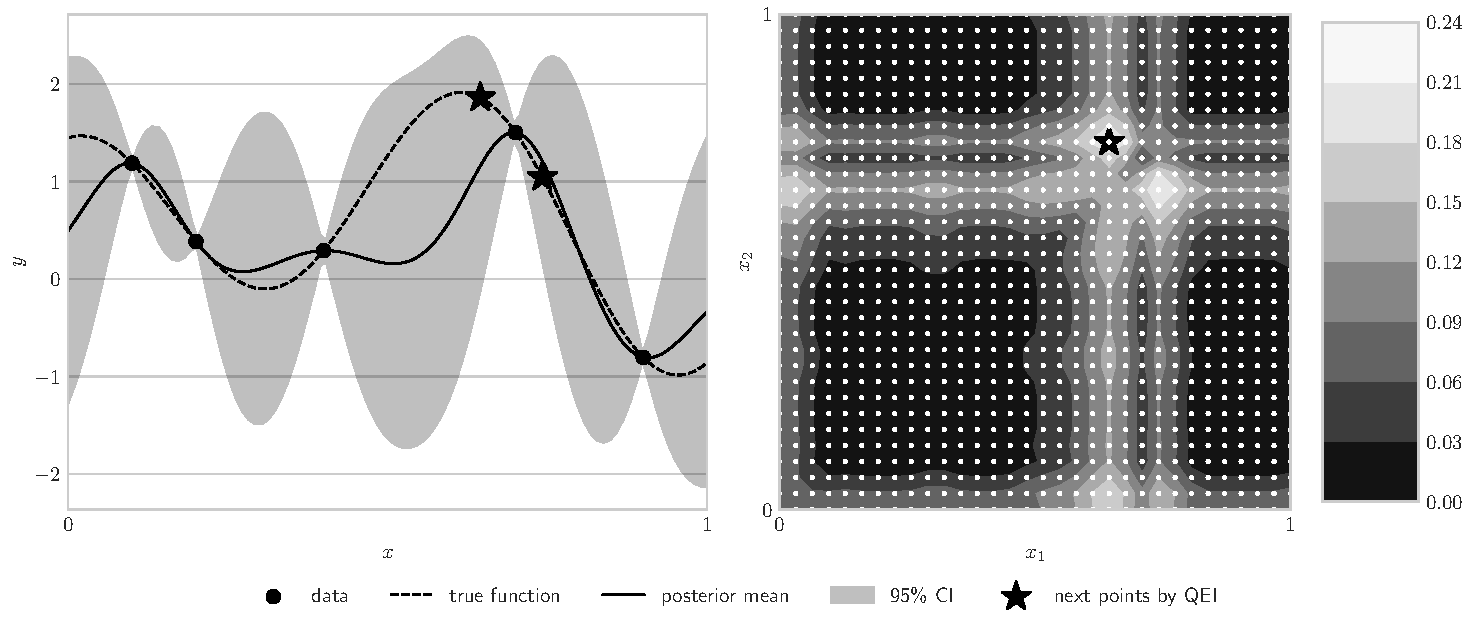
\includegraphics[width=\textwidth]{figs/gp.pdf}
    \caption{First, the true function has been sampled at the data points shown in the left panel. Next, a Gaussian Process is fit to the data points to approximate the true function. The posterior mean and $95\%$ confidence interval (CI) of the Gaussian Process are shown in the left panel. With $q=2$, a fine grid of candidates is chosen in $[0,1]^{2}$ and depicted in the right panel. The vectorized MC algorithm is then used to approximate the acquisition function value at each of the candidate grid points. These approximations are made into a contour plot in the right panel. The discrete argument maximum among these approximations on the fine grid is the next size $q$ batch of points by QEI. These next points for sequential optimization are visualized in both the right and left panels. }
    \label{SoRa_fig:bo_qei}
\end{figure}

\subsection{Bayesian Posterior Mean}

The Bayesian framework combines prior knowledge of unknown parameters $\boldsymbol{\Theta}$ with observational data and a likelihood function $\rho$ to construct an informed, model-aware posterior distribution on $\boldsymbol{\Theta}$. Suppose we have a dataset of observations $\boldsymbol{y} = (y_1,\dots,y_{N})$ taken at IID locations $\boldsymbol{z}_1,\dots,\boldsymbol{z}_{N}$ respectively. Then Bayes' rule may be used to write the posterior density of $\boldsymbol{\Theta}$ as 
$$P\left(\boldsymbol{\theta} \mid \boldsymbol{y} \right) = \frac{P(\boldsymbol{y} \mid \boldsymbol{\theta}) P(\boldsymbol{\theta})}{P\left(\boldsymbol{y}\right)} = \frac{\prod_{i=1}^{N} \rho(y_i \mid \boldsymbol{\theta}) P(\boldsymbol{\theta})}{\mathbb{E}\left[\prod_{i=1}^{N} \rho(y_i \mid \boldsymbol{\theta})\right]}.$$
Here the expectation is taken with respect to the prior distribution on $\boldsymbol{\Theta}$ with density $P(\boldsymbol{\theta})$, and $P\left(\boldsymbol{y} \mid \boldsymbol{S} \right)$ is the likelihood density which factors into the product of likelihoods $\rho(y_i \mid \boldsymbol{S})$ since the observations are IID. 

A useful quantity of interest is the posterior mean of $\boldsymbol{\Theta}$. In this example, the posterior mean is our combined solution $\boldsymbol{s}$ which may be written as the ratio of expectations via $\boldsymbol{s} = \mathbb{E}\left[\boldsymbol{\Theta} \mid \boldsymbol{y}\right] = \mathbb{E}\left[\boldsymbol{\Theta} \prod_{i=1}^{N} \rho(y_i \mid \boldsymbol{\Theta})\right]/\mathbb{E}\left[\prod_{i=1}^{N} \rho(y_i \mid \boldsymbol{\Theta})\right]$. As before, the expectations are taken with respect to the prior distribution on $\boldsymbol{\Theta}$. In the framework of this article $\boldsymbol{\mu} \in \mathbb{R}^{(2, d_{\boldsymbol{s}})}$ where for $k=1,\dots,d_{\boldsymbol{s}}$ we have 
$$\mu_{0k} = \mathbb{E}\left[\Theta_k \prod_{i=1}^{N} \rho(y_i \mid \boldsymbol{\Theta})\right], \qquad \mu_{1k} = \mathbb{E}\left[\prod_{i=1}^{N} \rho(y_i \mid \boldsymbol{\Theta})\right], \qquad \text{and} \qquad s_k = \frac{\mu_{0k}}{\mu_{1k}}.$$
Defining $\boldsymbol{C}^-$ and $\boldsymbol{C}^+$ follow from vectorizing the quotient forms in Table \ref{SoRa_table:elementary_ops_Cpm} while the dependency function $\boldsymbol{D}: \{\text{True},\text{False}\}^{d_{\boldsymbol{s}}} \to \{\text{True},\text{False}\}^{(2, d_{\boldsymbol{s}})}$ is defined by stacking the row vectors of combined flag on top of itself. While $\mu_{1k}$ is the same for all $1 \leq k \leq d_{\boldsymbol{s}}$, we opt to keep separate denominator estimates for each coefficient. Maintaining only a single estimate of $\mathbb{E}\left[\prod_{i=1}^{N} \rho(y_i \mid \boldsymbol{\Theta})\right]$ would require a different dependency function which removes economic function evaluation in favor of reduced storage. 

% Consider Bayesian logistic regression as a concrete example. Here the dataset contains observations $y_i \in \{0,1\}$ at locations $\boldsymbol{z}_i = \left(z_{i1},\dots,z_{i(d_{\boldsymbol{s}}-1)},1\right)$ for $i=1,\dots,N$ where the last value is $1$ to accommodate an intercept term. The sigmoid likelihood function $\rho(y_i = 1 \mid \boldsymbol{\theta}) = \frac{\exp(\boldsymbol{\theta}.\boldsymbol{z}_i)}{1+\exp(\boldsymbol{\theta}.\boldsymbol{z}_i)}$ may be used to yield
% $$P(\boldsymbol{y} \mid \boldsymbol{\theta}) = \prod_{i=1}^N \left(\frac{\exp(\boldsymbol{\theta}.\boldsymbol{z}_i)}{1+\exp(\boldsymbol{\theta}.\boldsymbol{z}_i)}\right)^{y_i} \left(1-\frac{\exp(\boldsymbol{\theta}.\boldsymbol{z}_i)}{1+\exp(\boldsymbol{\theta}.\boldsymbol{z}_i)}\right)^{1-y_i} = \prod_{i=1}^N \frac{\exp(\boldsymbol{\theta}.\boldsymbol{z}_i)^{y_i}}{1+\exp(\boldsymbol{\theta}.\boldsymbol{z}_i)}.$$

% Listing \ref{py:blr} performs Bayesian logistic regression in QMCPy
% %on the Haberman's Survival Dataset retrieved from the UCI Machine Learning Repository \cite{uci_ml_repo}
% . Here we use a normal prior $\boldsymbol{\Theta} \sim \mathcal{N}(\boldsymbol{m},\boldsymbol{\Sigma})$ so that
% $$P(\boldsymbol{\theta}) = \frac{\exp\left(-(\boldsymbol{\theta}-\boldsymbol{m})^T\boldsymbol{\Sigma}^{-1}(\boldsymbol{\theta}-\boldsymbol{m})/2\right)}{\sqrt{(2\pi)^d\lvert \det(\boldsymbol{\Sigma})\rvert }}.$$
% This example uses the absolute and relative error metric \eqref{SoRa_eq:h_abs_and_rel}. Notice that the number of samples required to approximate each coefficient is different. 
% \lstinputlisting[caption={Bayesian Logistic Regression},style=Python,label={py:blr}]{python/blr.txt}

\subsection{Sensitivity Indices}

Sensitivity analysis quantifies how uncertainty in a functions output may be attributed to subsets of function inputs. Functional ANOVA (analysis of variance) decomposes a function $\varphi \in L^2(0,1)^{d}$ into the sum of orthogonal functions $(\varphi_u)_{u \subseteq {1:d}}$. Here $1:d=\{1,\dots,d\}$ denotes the set of all dimensions and $\varphi_u \in L^2(0,1)^{\lvert u \rvert}$ denotes a sub-function dependent only on inputs $\boldsymbol{x}_u = (x_j)_{j \in u}$ where $\lvert u \rvert$ is the cardinality of $u$. By construction, these sub-functions sum to the objective function so that $\varphi(\boldsymbol{x}) = \sum_{u \subseteq 1:d} \varphi_u(\boldsymbol{x}_u)$ \cite[Appendix A]{mcbook}. The orthogonality of sub-functions enables the variance of $\varphi$ to be decomposed into the sum of variances of sub-functions. Specifically, denoting the variance of $\varphi$ by $\sigma^2$, we may write $\sigma^2 = \sum_{u \subseteq 1:d} \sigma^2_u$ where $\sigma^2_u$ is the variance of sub-function $\varphi_u$. The sub-variance $\sigma_u$ quantifies the variance of $\varphi$ attributable to inputs $u \subseteq 1:d$.  The \emph{closed, total Sobol' indices}
\begin{align*}
    \underline{\tau}_u^2 &= \sum_{v \subseteq u} \sigma^2_v = \int_{[0,1]^{2d}} f(\boldsymbol{x})[f(\boldsymbol{x}_{u_j},\boldsymbol{z}_{-{u_j}})-f(\boldsymbol{z})]\mathrm{d}\boldsymbol{x}\mathrm{d}\boldsymbol{z}, \\ 
    \overline{\tau}_u^2 &= \sum_{v \cap u \neq \emptyset} \sigma^2_v = \frac{1}{2}\int_{[0,1]^{2d}} [f(\boldsymbol{z})-f(\boldsymbol{x}_u,\boldsymbol{z}_{-{u_j}})]^2\mathrm{d}\boldsymbol{x}\mathrm{d}\boldsymbol{z}
    \label{SoRa_eq:sobol_indices}
\end{align*}
quantify the variance attributable to subsets of $u$ and subsets containing $u$ respectively. Here the notation $(\boldsymbol{x}_{u},\boldsymbol{z}_{-u})$ denotes a point where the value at index $1 \leq j \leq d$ is $x_j$ if $j \in u$ and $z_j$ otherwise. The \emph{closed, total sensitivity indices} $\underline{s}_u = \underline{\tau}_u^2/\sigma^2$, $\overline{s}_u = \overline{\tau}_u^2/\sigma^2$ normalize the Sobol' indices to quantify the proportion of variance explained by a given subset of inputs. 

Suppose one is interested in computing the closed and total sensitivity indices of $\varphi$ at $u_1,\dots,u_c \subseteq 1:d$. Then we may choose the individual solutions $\boldsymbol{\mu} \in \mathbb{R}^{(2, 3, c)}$ so that
%for $j=1,\dots,c$
% \begin{equation}
% \begin{aligned}
%     \mu_{11j} &= \underline{\tau}_{u_j}^2 = \int_{[0,1]^{2d}} f(\boldsymbol{x})[f(\boldsymbol{x}_{u_j},\boldsymbol{z}_{-{u_j}})-f(\boldsymbol{z})]\mathrm{d}\boldsymbol{x}\mathrm{d}\boldsymbol{z} \\
%     \mu_{21j} &= \overline{\tau}_{u_j}^2 = \frac{1}{2}\int_{[0,1]^{2d}} [f(\boldsymbol{z})-f(\boldsymbol{x}_u,\boldsymbol{z}_{-{u_j}})]^2\mathrm{d}\boldsymbol{x}\mathrm{d}\boldsymbol{z} \\
%     \mu_{12j} &= \mu_{22j} = \int_{[0,1]^{d}} f(\boldsymbol{x})\mathrm{d}\boldsymbol{x}, \\
%     \mu_{13j} &= \mu_{23j} = \int_{[0,1]^{d}} f^2(\boldsymbol{x})\mathrm{d}\boldsymbol{x}, \\
%     s_{1j} &= \underline{s}_{u_j} = \frac{\underline{\tau}_{u_j}^2}{\sigma^2} = \frac{\mu_{11j}}{\mu_{13j}-\mu_{12j}^2}, \\
%     s_{2j} &= \overline{s}_{u_j} = \frac{\overline{\tau}_{u_j}^2}{\sigma^2} = \frac{\mu_{21j}}{\mu_{23j}-\mu_{22j}^2}.  
% \end{aligned}
% \label{SoRa_eq:mu_si}
% \end{equation}
% In \eqref{SoRa_eq:mu_si}, 
$\boldsymbol{\mu}_1,\boldsymbol{\mu}_2 \in \mathbb{R}^{(3,c)}$ contain values for the closed, total sensitivity indices. Specifically,  $\boldsymbol{\mu}_{11},\boldsymbol{\mu}_{21} \in \mathbb{R}^c$ contain the closed, total Sobol' indices while $\boldsymbol{\mu}_{i2}, \boldsymbol{\mu}_{i3} \in \mathbb{R}^c$ contain first, second moments for any $i \in \{1,2\}$. For the combined solutions $\boldsymbol{s} \in \mathbb{R}^{(2, c)}$, we set $\boldsymbol{s}_1, \boldsymbol{s}_2 \in \mathbb{R}^c$ to contain the closed, total sensitivity indices. 

Bounds from individual to combined solutions may be propagated via $\boldsymbol{C}^-,\boldsymbol{C}^+:\mathbb{R}^{(2, 3, c)} \to \mathbb{R}^{(2, c)}$ defined for $i \in \{1,2\}$ and $j \in \{1,\dots,c\}$  by  
\begin{align*}
    C_{ij}^-(\boldsymbol{\mu}^-,\boldsymbol{\mu}^+) 
    %= \text{clip}\left(\min_{\boldsymbol{\mu} \in [\boldsymbol{\mu}^-,\boldsymbol{\mu}^+]} \frac{\mu_{i1j}}{\mu_{i3j}-\mu_{i2j}^2}\right) \\
    = \begin{cases} 
        \text{clip}\left(\min\left(\frac{\mu_{i1j}^-}{\mu_{i3j}^+-\left(\mu_{i2j}^-\right)^2},\frac{\mu_{i1j}^-}{\mu_{i3j}^+-\left(\mu_{i2j}^+\right)^2}\right)\right), & \mu_{i3j}^- - \left(\mu_{i2j}^\pm\right)^2 >0 \\
        0, &\text{else}
     \end{cases} %\\
    % C_{ij}^+(\boldsymbol{\mu}^-,\boldsymbol{\mu}^+) 
    % &= \text{clip}\left(\max_{\boldsymbol{\mu} \in [\boldsymbol{\mu}^-,\boldsymbol{\mu}^+]} \frac{\mu_{i1j}}{\mu_{i3j}-\mu_{i2j}^2}\right) \\
    % &= \begin{cases} 
    %     \text{clip}\left(\max\left(\frac{\mu_{i1j}^+}{\mu_{i3j}^--\left(\mu_{i2j}^-\right)^2},\frac{\mu_{i1j}^+}{\mu_{i3j}^--\left(\mu_{i2j}^+\right)^2}\right)\right), & \mu_{i3j}^- - \left(\mu_{i2j}^\pm\right)^2 >0 \\
    %     1, &\text{else}
    % \end{cases}
\end{align*}
with $C^+_{ij}(\boldsymbol{\mu}^-,\boldsymbol{\mu}^+)$ defined similarly and where $\text{clip}(\cdot) = \min(1,\max(0,\cdot))$ restricts values between 0 and 1. Above we have encoded the facts that sensitivity indices are between $0$ and $1$, the variance of $\varphi$ is non-negative, and Sobol' indices are non-negative. The dependency function $\boldsymbol{D}:\{\text{True},\text{False}\}^{(2, c)} \to \{\text{True},\text{False}\}^{(2, 3, c)}$ may be defined by broadcasting shapes so that for any $(1,1,1) \leq (i,j,k) \leq (2,3,c)$ we have $D_{ikj}(\boldsymbol{b}^{(\boldsymbol{s})}) = b_{ij}^{(\boldsymbol{s})}$. 

The QMCPy implementation further generalize to allow objective functions $\boldsymbol{\varphi}: (0,1)^{d} \to \mathbb{R}^{\tilde{\boldsymbol{d}}_{\boldsymbol{\mu}}}$ so that $\boldsymbol{d}_{\boldsymbol{\mu}} = (2,3,c,\tilde{\boldsymbol{d}}_{\boldsymbol{\mu}})$ and $\boldsymbol{d}_{\boldsymbol{s}} = (2,c,\tilde{\boldsymbol{d}}_{\boldsymbol{\mu}})$. Here the notation of nested vectors mean, for example, that  $(2,c,(5,6)) =(2,c,5,6)$.

Sensitivity indices present an important special case for computational complexity. Say our QMC algorithm takes $2^m$ total samples to accurately approximate closed and total sensitivity indices for $u_1,\dots,u_c \subseteq 1:d$. Then the computational cost is $\$(\boldsymbol{\varphi})(2+c)2^m$ since every time our sensitivity index function is evaluated at $(\boldsymbol{x},\boldsymbol{z}) \in [0,1]^{2d}$ we must evaluate the users objective function at $\boldsymbol{x}$, $\boldsymbol{z}$, and $(\boldsymbol{x}_{u_j},\boldsymbol{z}_{-{u_j}})$ for $j=1,\dots,c$. Also note that when $\boldsymbol{\varphi}$ is defined to take samples in  $[0,1)^{d}$ to outcomes in $\mathbb{R}^{\tilde{\boldsymbol{d}}_{\boldsymbol{\mu}}}$, sensitivity index approximation requires a wrapper taking samples in $[0,1)^{2d}$ to outcomes in $\mathbb{R}^{\boldsymbol{d}_{\boldsymbol{\mu}}}$.

If a user is only interested in approximating singleton sensitivity indices, $u_j = \{j\}$ for $j=1,\dots,d$, then it is possible to reduce the cost from $\$(\boldsymbol{\varphi})(2+d)2^m$ to $\$(\boldsymbol{\varphi})2^{m+1}$ using order $1$ replicated designs \cite{alex2008comparison,tissot2015randomized}. Such designs have been extended to  digital sequences in \cite{replicated_designs_sobol_seq} and utilized for sensitivity index approximation in \cite{reliable_sobol_indices_approx}.

We first illustrate our vectorized (Q)MC algorithm by computing the sensitivity indices of the  Ishigami function \cite{ishigami1990importance} $g(\boldsymbol{T}) = (1+bT_3^4)\sin(T_1)+a\sin^2(T_2)$ where $\boldsymbol{T} \sim \mathcal{U}(-\pi,\pi)^3$ and $a=7$, $b=0.1$ as in \cite{crestaux2007polynomial,marrel2009calculations}. Figure \ref{SoRa_fig:ishigami} visualizes the resulting optimal approximations and combined error bounds which capture the exact sensitivity indices of the Ishigami function. 

\begin{figure}[t]
    \centering
    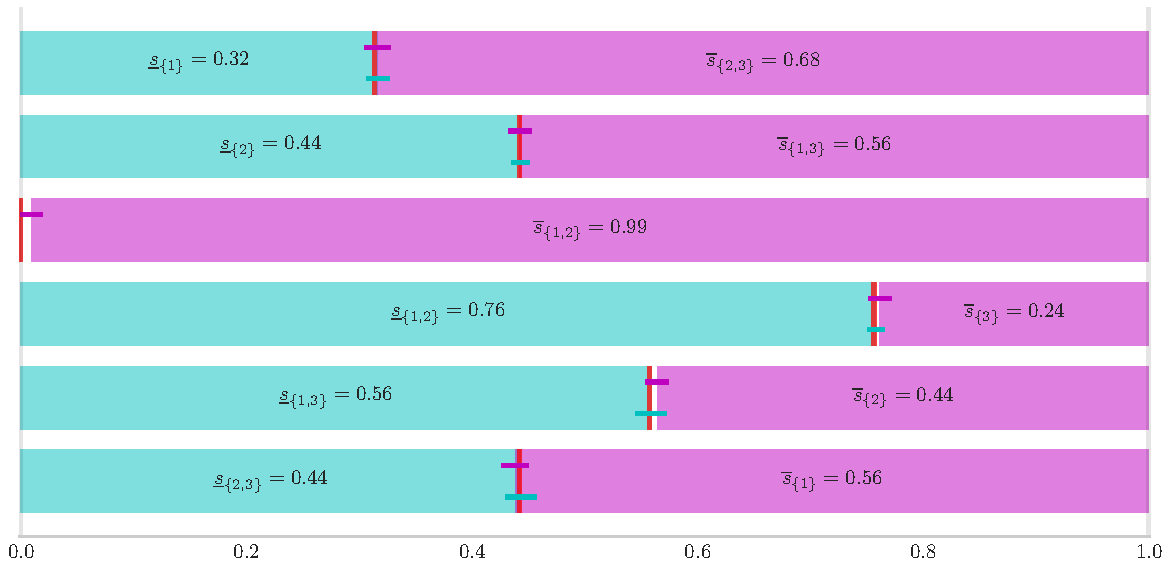
\includegraphics[width=.8\textwidth]{figs/ishigami.pdf}
    \caption{Approximate closed and total sensitivity indices for the Ishigami function illustrating the relationship $\underline{s}_u + \overline{s}_{u^c} = 1$ for all $u \subseteq 1:d$. In each row the closed sensitivity index bar is  extended to the right from $0$ while the total sensitivity index bar is extended to the left from $1$. The bars should meet at the heavy vertical line for the analytic solution $\underline{s}_u=1-\overline{s}_{u^c}$. The darker, lighter horizontal lines within each row depict the error bounds for the closed, total sensitivity indices respectively. The heavy vertical line crossing both horizontal lines in each row indicates the true solution is indeed captured in the error bounds.}
    \label{SoRa_fig:ishigami}
\end{figure}

In another example, we compute sensitivity indices of a neural network classifier \cite{he2015delving} for the Iris dataset \cite{uci_ml_repo}. This example was inspired by a similar experiment in \cite{hoyt2021efficient}. The dataset consists of attributes sepal length (\textbf{SL}), sepal width (\textbf{SW}), petal length (\textbf{PL}), and petal width (\textbf{PW}), all in centimeters, from which an Iris is to be classified as either the \emph{setosa}, \emph{versicolor}, or \emph{virginica} species. We begin by fitting a neural network classifier which takes in input features and outputs a size $3$ vector of probabilities for each species summing to $1$. Taking the argument maximum among these three probabilities gives a species prediction. On a held out portion of the dataset the neural network attains 98\% classification accuracy and may therefore be deemed a high quality surrogate for the true relation between input features and species classification. 

Our problem is to quantify, for each species, the variability in the classification probability attributed to a set of inputs. In other words, we would like to compute the sensitivity indices for each species probability. 
%In Listing \ref{py:nn} below we compute all sensitivity indices with the help of the scikit-learn package \cite{scikit-learn} for splitting off a holdout dataset and training the neural network classifier. 
Here $\boldsymbol{d}_{\boldsymbol{\mu}} = (2,3,14,3)$ and $\boldsymbol{d}_{\boldsymbol{s}} = (2,14,3)$ since we have $3$ species classes, $14$ sensitivity indies of interest, and we are computing both the closed and total sensitivity indices. Figure \ref{SoRa_fig:nn_si} visualizes closed sensitivity index approximations. 
%\lstinputlisting[caption={Neural Network Sensitivity Indices},style=Python,label={py:nn}]{python/nn.txt}

\begin{figure}[t]
    \centering
    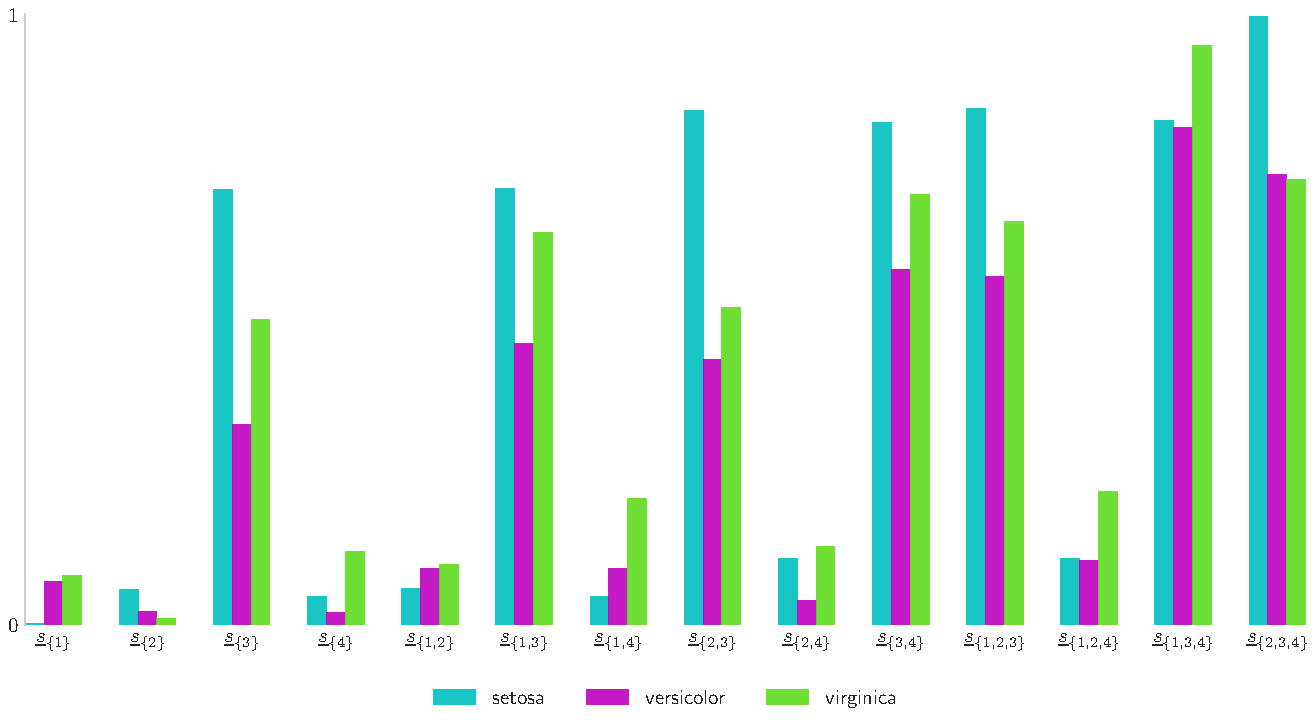
\includegraphics[width=.8\textwidth]{figs/nn_si.pdf}
    \caption{Closed sensitivity indices for neural network classification probability of each Iris species.}
    \label{SoRa_fig:nn_si}
\end{figure}

\section{Conclusion} \label{SoRa_sec:conclusions}

This article has extended adaptive MC and QMC stopping criteria to support approximating multi-dimensional quantities of interest formulated as functions of multi-dimensional expectations. The resulting method is compatible with algorithms providing error bounds which hold with a desired uncertainty based on function evaluations at IID or LD sequences. Our work has been implemented into the open-source QMCPy package and exemplified on problems in machine learning and global sensitivity analysis. 

%\printbibliography
%\section*{References}
%\nocite{*}
%\bibliographystyle{spmpsci.bst}
%\bibliography{ags,main}
%\bibliography{main}

\begin{thebibliography}{10}
\providecommand{\url}[1]{{#1}}
\providecommand{\urlprefix}{URL }
\expandafter\ifx\csname urlstyle\endcsname\relax
  \providecommand{\doi}[1]{DOI~\discretionary{}{}{}#1}\else
  \providecommand{\doi}{DOI~\discretionary{}{}{}\begingroup
  \urlstyle{rm}\Url}\fi

\bibitem{qmc4pde}Kuo, F. \& Nuyens, D. Application of quasi-Monte Carlo methods to elliptic PDEs with random diffusion coefficients: a survey of analysis and implementation. {\em Foundations Of Computational Mathematics}. \textbf{16}, 1631-1696 (2016)

\bibitem{cubqmcbayeslattice}
Fast automatic Bayesian cubature using lattice sampling \textbf{29}

\bibitem{replicated_designs_sobol_seq}
Iterative construction of replicated designs based on sobol' sequences.
\newblock Comptes Rendus Mathematique \textbf{355}(1), 10--14 (2017)

\bibitem{alex2008comparison}
Alex~Mara, T., Rakoto~Joseph, O.: Comparison of some efficient methods to
  evaluate the main effect of computer model factors.
\newblock Journal of Statistical Computation and Simulation \textbf{78}(2),
  167--178 (2008)

\bibitem{boole1847mathematical}
Boole, G.: The mathematical analysis of logic.
\newblock Philosophical Library (1847)

\bibitem{ChoEtal21a}
Choi, S.C.T., Ding, Y., Hickernell, F.J., Jiang, L., {Jim\'enez Rugama},
  {\relax Ll}.A., Li, D., Jagadeeswaran, R., Tong, X., Zhang, K., Zhang, Y.,
  Zhou, X.: {GAIL}: {G}uaranteed {A}utomatic {I}ntegration {L}ibrary (versions
  1.0--2.3.2).
\newblock MATLAB software, \url{http://gailgithub.github.io/GAIL\_Dev/} (2021).
\newblock \doi{10.5281/zenodo.4018189}

\bibitem{QMCPy}
Choi, S.C.T., Hickernell, F.J., Jagadeeswaran, R., McCourt, M.J., Sorokin,
  A.G.: {QMCPy}: A {Q}uasi-{M}onte {C}arlo {P}ython library (2022).
\newblock \urlprefix\url{https://github.com/QMCSoftware/QMCSoftware}

\bibitem{QMCSoftware}
Choi, S.C.T., Hickernell, F.J., Jagadeeswaran, R., McCourt, M.J., Sorokin,
  A.G.: Quasi-monte carlo software.
\newblock In: A.~Keller (ed.) Monte Carlo and Quasi-Monte Carlo Methods, pp.
  23--47. Springer International Publishing, Cham (2022)

\bibitem{crestaux2007polynomial}
Crestaux, T., Martinez, J., Le~Maitre, J., Lafitte, O.: Polynomial chaos
  expansion for uncertainties quantification and sensitivity analysis
  [powerpoint slides]. retrieved from samo 2007 (2007)

\bibitem{dick2013high}
Dick, J., Kuo, F.Y., Sloan, I.H.: High-dimensional integration: the quasi-monte
  carlo way.
\newblock Acta Numerica \textbf{22}, 133--288 (2013)

\bibitem{uci_ml_repo}
Dua, D., Graff, C.: {UCI} machine learning repository (2017).
\newblock \urlprefix\url{http://archive.ics.uci.edu/ml}

\bibitem{frazier2018tutorial}
Frazier, P.I.: A tutorial on bayesian optimization.
\newblock arXiv preprint arXiv:1807.02811  (2018)

\bibitem{he2015delving}
He, K., Zhang, X., Ren, S., Sun, J.: Delving deep into rectifiers: Surpassing
  human-level performance on imagenet classification.
\newblock In: Proceedings of the IEEE international conference on computer
  vision, pp. 1026--1034 (2015)

\bibitem{hickernell1998generalized}
Hickernell, F.: A generalized discrepancy and quadrature error bound.
\newblock Mathematics of computation \textbf{67}(221), 299--322 (1998)

\bibitem{hickernell2018monte}
Hickernell, F.J., Choi, S.C.T., Jiang, L., Rugama, L.A.J.: Monte carlo
  simulation, automatic stopping criteria for.
\newblock Wiley StatsRef: Statistics Reference Online pp. 1--7 (2018)

\bibitem{cubmcg}
Hickernell, F.J., Jiang, L., Liu, Y., Owen, A.: Guaranteed conservative fixed
  width confidence intervals via monte carlo sampling (2012)

\bibitem{cubqmcsobol}
Hickernell, F.J., {Jim\'enez Rugama}, L.A.: Reliable adaptive cubature using
  digital sequences (2014)

\bibitem{adaptive_qmc}
Hickernell, F.J., Jim\'{e}nez~Rugama, L.A., Li, D.: Adaptive quasi-monte carlo
  methods for cubature.
\newblock In: Contemporary Computational Mathematics-A Celebration of the 80th
  Birthday of Ian Sloan, pp. 597--619. Springer (2018)

\bibitem{hoyt2021efficient}
Hoyt, C., Owen, A.B.: Efficient estimation of the anova mean dimension, with an
  application to neural net classification.
\newblock SIAM/ASA Journal on Uncertainty Quantification \textbf{9}(2),
  708--730 (2021)

\bibitem{ishigami1990importance}
Ishigami, T., Homma, T.: An importance quantification technique in uncertainty
  analysis for computer models.
\newblock In: [1990] Proceedings. First International Symposium on Uncertainty
  Modeling and Analysis, pp. 398--403. IEEE (1990)

\bibitem{reliable_sobol_indices_approx}
Jim{\'e}nez~Rugama, L.A., Gilquin, L.: {Reliable error estimation for Sobol'
  indices}.
\newblock {Statistics and Computing} \textbf{28}(4), 725--738 (2018).
\newblock \urlprefix\url{https://hal.inria.fr/hal-01358067}

\bibitem{cubqmclattice}
{Jim\'enez Rugama}, L.A., Hickernell, F.J.: Adaptive multidimensional
  integration based on rank-1 lattices (2014)

\bibitem{marrel2009calculations}
Marrel, A., Iooss, B., Laurent, B., Roustant, O.: Calculations of sobol indices
  for the gaussian process metamodel.
\newblock Reliability Engineering \& System Safety \textbf{94}(3), 742--751
  (2009)

\bibitem{interval_analysis}
Moore, R.E., Kearfott, R.B., Cloud, M.J.: Introduction to interval analysis.
\newblock SIAM (2009)

\bibitem{niederreiter1992random}
Niederreiter, H.: Random number generation and quasi-Monte Carlo methods.
\newblock SIAM (1992)

\bibitem{mcbook}
Owen, A.B.: Monte Carlo theory, methods and examples (2018)

\bibitem{cubqmcbayes_thesis}
Rathinavel, J.: {F}ast automatic {B}ayesian cubature using matching kernels and
  designs.
\newblock Phd thesis, Illinois Institute of Technology, Chicago (2019).
\newblock \urlprefix\url{www.math.iit.edu}

\bibitem{vectorized_qmc_demo_notebook}
Sorokin, A.G.: {M}onte {C}arlo for {V}ector {F}unctions of {I}ntegrals
  {R}eproducible {E}xamples (2022).
\newblock \urlprefix\url{https://qmcpy.readthedocs.io/en/latest/demo\_rst/vectorized\_qmc.html}

\bibitem{tissot2015randomized}
Tissot, J.Y., Prieur, C.: A randomized orthogonal array-based procedure for the
  estimation of first-and second-order sobol'indices.
\newblock Journal of Statistical Computation and Simulation \textbf{85}(7),
  1358--1381 (2015)

\end{thebibliography}


% BEGIN TO REMOVE
\iffalse
\section*{TODO}

\subsection*{Article}

\begin{itemize}
    \item \AGSComment{Add future work to conclusion}
    \item \JRComment{Is there any default recommendation if the user does not have any knowledge about the integrand?}
    \item \JRComment{Please mention any prior work in vectorized Monte Carlo}
    \item \FJHComment{To cut down on the number of pages, you may want to refer readers to a demo of your code on the QMCPy website.  The editors may have trouble compiling the LaTeX of the book with your source code listings definitions.}
    \item \AGSComment{Remove extra macros e.g. bib stuff and comment commands}
    \item \AGSComment{remove TODO section and table of contents from the end}
\end{itemize}

\subsection*{Code}

\begin{itemize}
    \item \AGSComment{\texttt{CubBayes} algorithms allow ndarray of \texttt{abs\_tol} and \texttt{rel\_tol} and \texttt{error\_fun}}
    \item \AGSComment{Ensure paper code matches notebook code after all changes}
    \item \AGSComment{New PyPI release}
\end{itemize}

\subsection*{To Review}

\begin{itemize}
    \item \FJHComment{It would help to have a connecting sentence or two at the start and/or end of each section to tell the reader where you are going next.}
    \item \FJHComment{You may want to start importing this into the conference proceedings styles so that you can adapt to them sooner rather than later.}
    \item \FJHComment{It is better not to have just one subsubsection of a subsection.}
\end{itemize}

\tableofcontents
\fi
% END TO REMOVE

\end{document}
